\section{Coeficientes de Fourier como sistemas dinámicos}
\begin{frame}
    \frametitle{Coeficientes de Fourier como sistemas dinámicos}
    \begin{itemize}
        \item Mediante el teorema fundamental de cálculo transformarmos la integrales en ecuaciones diferenciales, de la siguiente manera:
    \end{itemize}
    \begin{gather}
        \alpha_i(\tau) = \frac{2}{\pi}\int_0^\tau f(\tau) \sin(i\tau)d\tau 
        \Rightarrow
        \begin{cases} \label{ode}
            \dot{\alpha_i}(\tau) & = \frac{2}{\pi}f(\tau)\sin(i\tau) \\  
            \alpha_i(0) & = 0       
        \end{cases}
    \end{gather}
    
    \begin{gather}
        \beta_j(\tau) = \frac{2}{\pi}\int_0^\tau f(\tau) \cos(j\tau)d\tau 
        \Rightarrow
        \begin{cases} \label{ode}
            \dot{\beta}_j(\tau) & = \frac{2}{\pi}f(\tau)\cos(j\tau) \\  
            \beta_j(0) & = 0       
        \end{cases}
    \end{gather}

\end{frame}
%%%%%%%%%%%%%%%%%%%%%%%%%%%%%%%%%%%%%%%%%%%%%%%
\begin{frame}
    \frametitle{Coeficientes de Fourier como sistemas dinámicos}
    
    \begin{itemize}
        \item De esta manera, el estado $\{ \alpha_{i},\beta_{j} \}$ en el intante de tiempo $\tau = \pi$ son los coeficientes de Fourier de $f(\tau) $
    \end{itemize}
    \begin{gather}
        \begin{cases} \label{ode}
            \dot{\alpha_i}(\tau) & = \frac{2}{\pi}f(\tau)\sin(i\tau) \\  
            \alpha_i(0) & = 0       
        \end{cases}
        \Rightarrow 
        \alpha_i(\pi) = a_i^T
    \end{gather}
    
    \begin{gather}
        \begin{cases} 
            \dot{\beta}_j(\tau) & = \frac{2}{\pi}f(\tau)\cos(j\tau) \\  
            \beta_j(0) & = 0       
        \end{cases}
        \Rightarrow 
        \beta_i(\pi) = b_i^T
    \end{gather}
    Entonces el problema se traduce a encontrar un control $f(t)$ que conduzca al sistema desde el origen de coordenadas hasta el punto objetivo marcado.
\end{frame}
%%%%%%%%%%%%%%%%%%%%%%%%%%%%%%%%%%%%%%%%%%%%%%%
\begin{frame}
    \frametitle{Coeficientes de Fourier como sistemas dinámicos}
    
    \begin{itemize}
        \item Consideramos los conjuntos $\mathcal{E}_a = {1}$ y $\mathcal{E}_b = {1}$
        \item El sistema dinámico se escribe como:
        \begin{gather}
            \begin{cases} 
                \dot{\alpha}_1(\tau) & = \frac{2}{\pi}f(\tau)\sin(\tau) \ | \  \alpha(0) = 0\\
                \dot{\beta}_1(\tau) & = \frac{2}{\pi}f(\tau)\cos(\tau)  \ | \  \beta(0) = 0
            \end{cases}  
        \end{gather}

        \item Si aplicamos $f(\tau)$ al sistema $(\alpha_1(\tau),\beta_1(\tau))$, entonces el vector de estado final 
        \begin{gather}
            (\alpha_1(\pi),\beta_1(\pi)) = (a_1,b_1) \text{ de } f(\tau)
        \end{gather}
    \end{itemize}
\end{frame}

\begin{frame}
    \frametitle{Coeficientes de Fourier como sistemas dinámicos}
    \begin{figure}
        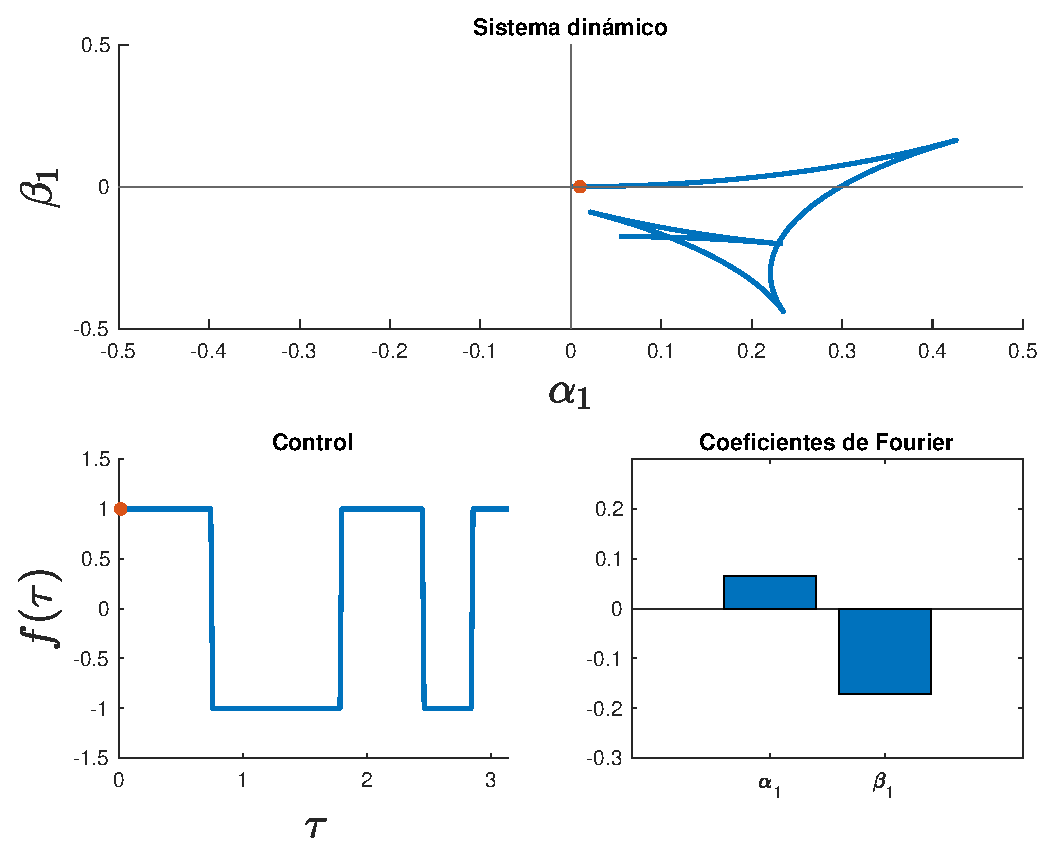
\includegraphics[scale=0.4]{imgs/S0001.eps}
        \caption{Evolución de un sistema $\{\alpha_1,\beta_1\}$ Sistema dinámico}
    \end{figure}
\end{frame}


%%%%%%%%%%%%%%%%%%%%%%%%%%%%%%%%%%%%%%%%%%%%%%%
